\header{
    \section{Les quatre-vingt chasseurs} \label{les-quatre-vingt-chasseurs}
    %
    
    \insertComment{Pastiche d'un poème de Victor Hugo (Indes orientales, 1828) datant de 1866.}{}
}

\begin{tikzpicture}[remember picture,overlay]
    \node[xshift=-3cm,yshift=-15cm] at (current page.north east){%
    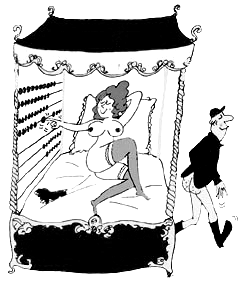
\includegraphics[width=0.4\textwidth]{images/chasseurs.png}};
\end{tikzpicture}
\enluminure{4}{\href{https://www.youtube.com/watch?v=hLXHcxWCQAI}{A}}{l'ouverture} de la chasse,
\\Dans un château riche en gibier, riche en gibier
\\Une marquise aux fins limiers
\\Invitation des chasseurs en masse.
\\Bientôt, l'on vit tous les chasseurs
\\Accourir sans mêm' qu'on leur dise.
\\\\\textbf{Refrain :}
\\Au rendez-vous de la Marquise,
\\Nous étions quatre-vingts chasseurs.
\\Au rendez-vous de la Marquise,
\\Nous étions quatre-vingts chasseurs,
\\80, 80, 80, 80 chasseurs
\\80, 80, 80, 80 chasseurs
\\\\"Allons, chasseurs, vite en campagne !
\\Dit la Marquise, Il faut partir ! Il faut partir !
\\Que chacun songe à son plaisir ;
\\Le son du cor nous accompagne."
\\Au bruit des chants et des clameurs
\\Plus d'une biche fut surprise...
\\\\\textbf{Refrain :}
\\Quand, dans les bois de la Marquise,..
\\\\Encouragés par notre belle,
\\Nous abattîm's plus d'un faisan;
\\Quand un sanglier menaçant
\\Vint à s'élancer sur elle.
\\Malgré sa rare et sa fureur,
\\Nous l'obligeâm's à lâcher prise;
\breakpage
\textbf{Refrain :}
\\Car pour défendre la Marquise,...
\\\\"Après s'être couvert de gloire,
\\Dit la Marquise, il faut rentrer ! Il faut rentrer !
\\Ce n'est pas tout de s'illustrer;
\\Il faut encore manger et boire !
\\Servez les mets et les liqueurs,
\\Et que la nappe soit bien mise!"
\\\\\textbf{Refrain :}
\\À la table de la Marquise,...
\\\\Quand nous eûmes savouré l'champagne,
\\Nous fûmes disposés à l'amour, oui, à l'amour.
\\Chacun voulut plaire à son tour
\\À notre illustre compagne.
\\Tous en obtinrent les faveurs
\\Car la noble dame était grise.
\\\\\textbf{Refrain :}
\\Et dans le lit de la Marquise,...
\\\\Ce fut une nuit mémorable.
\\La Marquise, neuf mois plus tard, neuf mois plus tard,
\\Mit au monde un joyeux bâtard,
\\Aujourd'hui tireur redoutable.
\\De ses jours, ignorant l'auteur
\\Il demanda qu'on l'en instruise.
\\\\\textbf{Refrain final :}]
\\\\"Tu es, lui dit notre Marquise,
\\L'enfant de quatre-vingts chasseurs
\\"Tu es, lui dit notre Marquise,
\\L'enfant de quatre-vingts chasseurs
\\80, 80, 80, 80 chasseurs
\\80, 80, 80, 80 chasseurs
\\Qui n'avaient pas peur".
%\enluminure{4}{A}{l'ouverture} de la chasse,
%\\Dans un château riche en gibier,
%\\Riche en gibier,
%\\Une marquise sans héritiers
%\\Invita des chasseurs en masse.
%\\Alors vit-on plus d'un chasseur,
%\\Accouru sans qu'on lui dise,
%\\Et à la chasse de la marquise,
%\\\\\textbf{Refrain :}
%Nous étions 80 chasseurs,
%\\80 80 80 80 chasseurs,
%\\80 80 80 80 chasseurs,
%\\Qui n'avions pas peur!
%\\\\Encouragés par notre belle,
%\\Nous abattions plus d'un faisan,
%\\Lorsqu'un sanglier effrayant
%\\Tout à coup s'élança sur elle:
%\\Malgré sa force et sa vigueur,
%\\Et pour défendre la marquise,
%\\Nous le forçâmes à lâcher prise.
%\\\\"Allons chasseurs, vite en campagne",
%\\Dit la marquise, "Il faut partir,
%\\Il suffit pas de se réjouir,
%\\Il faut encore manger et boire."
%\\Au milieu des champs et des cris
%\\La table fut aussitôt mise,
%\\Et à la table de la marquise,
%\\\\Lorsqu'on nous servit le champagne,
%\\Les coeurs se disposent à l'amour.
%\\Chacun voulut plaire à son tour
%\\A notre illustre compagne,
%\\Chacun d'elle obtint une faveur,
%\\Si bien que la dame était prise,
%\\Et dans le lit de la marquise,
%\\\\Pour fêter ce jour mémorable,
%\\La marquise neuf mois plus tard
%\\Mit au monde un jeune bâtard
%\\Qui aujourd'hui est redoutable.
%\\De sa force ignorant l'auteur,
%\\Il voulut qu'on l'en instruise.
%\\"Tu es", dit la marquise,
%\\\\\textbf{Refrain final :}
%\\"L'enfant des 80 chasseurs
%\\80 80 80 80 chasseurs,
%\\80 80 80 80 chasseurs,
%\\Qui n'avaient pas peur".

\breakpage